\documentclass[a4paper,12pt]{article}
\usepackage[margin=1in]{geometry} % 1-inch margins
\usepackage{tikz} % For the border
\usetikzlibrary{calc} % For coordinate calculations
\usepackage{graphicx} % For including the logo
\usepackage{lmodern} % Font package
\usepackage{titlesec} % Section formatting
\usepackage{fancyhdr} % Footer customization
\usepackage{amsmath}
\usepackage{listings}
\usepackage{caption}
\usepackage{subcaption}
\usepackage{geometry}
\usepackage{array}
\usepackage{booktabs}
\usepackage{makecell}
\usepackage{tocloft}
\usepackage[colorlinks=true, linkcolor=black, citecolor=black, urlcolor=black]{hyperref}
\usepackage{graphicx} % Required for inserting images
\usepackage{float} % Required for precise figure placement
\usepackage{listings}
\usepackage{color}
\usepackage{tikz}
\usetikzlibrary{shapes.geometric, arrows}

\tikzstyle{process} = [rectangle, minimum width=3cm, minimum height=1cm, text centered, draw=black, fill=blue!30]
\tikzstyle{arrow} = [thick,->,>=stealth]

\definecolor{dkgreen}{rgb}{0,0.6,0}
\definecolor{gray}{rgb}{0.5,0.5,0.5}
\definecolor{mauve}{rgb}{0.58,0,0.82}

\lstset{frame=tb,
  language=C,
  aboveskip=3mm,
  belowskip=3mm,
  showstringspaces=false,
  columns=flexible,
  basicstyle={\small\ttfamily},
  numbers=none,
  numberstyle=\tiny\color{gray},
  keywordstyle=\color{blue},
  commentstyle=\color{dkgreen},
  stringstyle=\color{mauve},
  breaklines=true,
  breakatwhitespace=true,
  tabsize=3
}

\definecolor{codegreen}{rgb}{0,0.6,0}
\definecolor{codegray}{rgb}{0.5,0.5,0.5}
\definecolor{codepurple}{rgb}{0.58,0,0.82}
\definecolor{backcolour}{rgb}{0.95,0.95,0.92}

\lstdefinestyle{mystyle}{
    backgroundcolor=\color{backcolour},   
    commentstyle=\color{codegreen},
    keywordstyle=\color{magenta},
    numberstyle=\tiny\color{codegray},
    stringstyle=\color{codepurple},
    basicstyle=\ttfamily\footnotesize,
    breakatwhitespace=false,         
    breaklines=true,                 
    captionpos=b,                    
    keepspaces=true,                 
    numbers=left,                    
    numbersep=5pt,  
    showlines=false,
    showspaces=false,                
    showstringspaces=false,
    showtabs=false,                  
    tabsize=2
}

\lstset{style=mystyle, showlines=false}

\begin{document}

% --- First Page Border ---
\begin{tikzpicture}[remember picture, overlay]
    \draw[line width=2pt]
        ($(current page.south west) + (0.5in, 0.5in)$) 
        rectangle 
        ($(current page.north east) - (0.5in, 0.5in)$);
\end{tikzpicture}

% --- University Name ---
\begin{center}
    \vspace{1cm}
    {\Large \textbf{University of Science and Technology of Hanoi}}\\[0.75cm]
    
    % --- University Logo ---
    \includegraphics[width=0.5\textwidth]{usth.png}
    
    \vspace{1cm}
    {\large \textbf{Distributed System}}\\[0.5cm]
    {\large \textbf{Midterm report}}\\[0.5cm]

    % --- Assignment Title ---
    \vspace{0.8cm}
    \rule{\textwidth}{0.75pt} \\[0.3cm]
    {\huge \textbf{HTTP over MPI}}\\[0.3cm]
    \rule{\textwidth}{0.75pt} \\[1.5cm]
\end{center}


% --- Student Information ---
\vspace{1cm}
\noindent
\begin{tabular}{>{\bfseries}l @{\hskip 0.5cm} c @{\hskip 0.5cm} l}
    Group       & : & \textit{09}\\[0.2cm]
    Members     & : & \textit{Nguyen Tai Anh - 22BI13028}\\[0.2cm]
                & : & \textit{Do Bao Nhi - 22BI13349}\\[0.2cm]
                & : & \textit{Do Trong Dat - 22BI13075}\\[0.2cm]
                & : & \textit{Hoang Quan - 22BI13368}\\[0.2cm]
                & : & \textit{Le Van Truong - 22BI13440}\\[0.2cm]
                & : & \textit{Nguyen Hai Nam - 22BI13322}\\[0.2cm]
    Major       & : & \textit{Cyber Security}             \\[0.2cm]
    Lecturer    & : & \textit{MSc. Le Nhu Chu Hiep}\\

\end{tabular}

\vfill

% --- Footer ---
\begin{center}
    \textit{Hanoi, December 31 2024}
\end{center}

\tableofcontents

\clearpage
\section{Introduction}
This report details an MPI (Message Passing Interface)-based system designed to send an HTTP request from a client process to a server via a proxy process. The client can either send a predefined message or the contents of a file. The proxy forwards the request to a specified HTTP server, retrieves the response, and sends it back to the client. This system employs MPI for message passing, making it suitable for parallel computing environments.

\section{System Overview}
The system involves two key processes:
\begin{itemize}
    \item \textbf{Client Process}: Sends an HTTP request to the proxy, either as a predefined message or the contents of a file.
    \item \textbf{Proxy Process}: Receives the HTTP request from the client, forwards it to an HTTP server (via libcurl), and sends the response back to the client.
\end{itemize}

The communication between the client and the proxy is managed via MPI. The client sends an HTTP request message, and the proxy forwards it to the HTTP server. The proxy then returns the server's response to the client.

\section{MPI (Message Passing Interface) Overview}
\begin{table}[h!]
\centering
\begin{tabular}{|l|l|}
\hline
\textbf{Primitive}    & \textbf{Meaning}                                                                   \\ \hline
\texttt{MPI\_bsend}    & Append outgoing message to a local send buffer                                    \\ \hline
\texttt{MPI\_send}     & Send a message and wait until copied to local or remote buffer                    \\ \hline
\texttt{MPI\_ssend}    & Send a message and wait until receipt starts                                      \\ \hline
\texttt{MPI\_sendrecv} & Send a message and wait for reply                                                 \\ \hline
\texttt{MPI\_isend}    & Pass reference to outgoing message, and continue                                  \\ \hline
\texttt{MPI\_issend}   & Pass reference to outgoing message, and wait until receipt starts                \\ \hline
\texttt{MPI\_recv}     & Receive a message; block if there is none                                         \\ \hline
\texttt{MPI\_irecv}    & Check if there is an incoming message, but do not block                           \\ \hline
\end{tabular}
\caption{MPI Primitives and their Meanings}
\label{table:mpi_primitives}
\end{table}
\noindent
MPI is a standardized and portable message-passing system designed for parallel computing. It enables processes to communicate with each other by sending and receiving messages. This system uses MPI for inter-process communication, specifically:
\begin{itemize}
    \item \textbf{MPI\_Send}: Used by the client to send the HTTP request to the proxy.
    \item \textbf{MPI\_Recv}: Used by the proxy to receive the HTTP request from the client, and by the client to receive the HTTP response from the proxy.
\end{itemize}

\subsection{Key MPI Functions Used}
\begin{itemize}
    \item \textbf{MPI\_Init}: Initializes the MPI environment.
    \item \textbf{MPI\_Comm\_rank}: Determines the rank of the process in the communicator.
    \item \textbf{MPI\_Comm\_size}: Determines the size of the communicator (number of processes).
    \item \textbf{MPI\_Send} and \textbf{MPI\_Recv}: Used for sending and receiving data.
\end{itemize}
\begin{table}[h!]
\centering
\begin{tabular}{|p{4cm}|p{10cm}|}
\hline
\textbf{MPI Function}  & \textbf{Purpose}                                                                                   \\ \hline
\texttt{MPI\_Init}     & Initializes the MPI environment.                                                                   \\ \hline
\texttt{MPI\_Comm\_rank} & Determines the rank (ID) of the current process within the MPI communicator.                      \\ \hline
\texttt{MPI\_Comm\_size} & Determines the total number of processes in the MPI communicator.                                 \\ \hline
\texttt{MPI\_Send}     & Sends a message (data) from one process to another.                                                \\ \hline
\texttt{MPI\_Recv}     & Receives a message (data) from another process.                                                    \\ \hline
\texttt{MPI\_Abort}    & Aborts all MPI processes in the communicator if an error occurs.                                   \\ \hline
\texttt{MPI\_Finalize} & Terminates the MPI environment, cleaning up resources used by MPI.                                 \\ \hline
\end{tabular}
\caption{Common MPI Functions and their Purposes}
\label{table:mpi_functions}
\end{table}


\section{System Architecture}
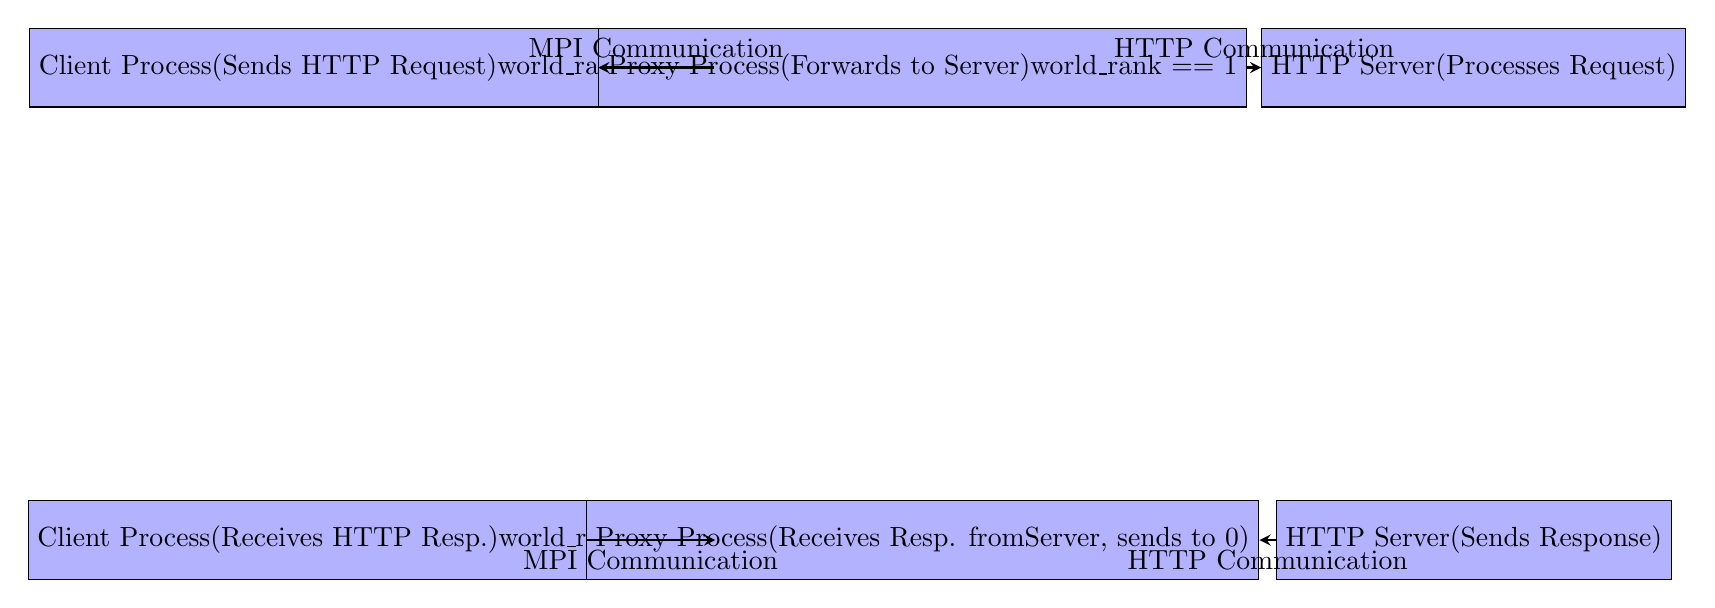
\begin{tikzpicture}[node distance=3cm]

% Nodes
\node (client) [process] {Client Process \\ (Sends HTTP Request) \\ world\_rank == 0};
\node (proxy) [process, right of=client, xshift=4cm] {Proxy Process \\ (Forwards to Server) \\ world\_rank == 1};
\node (server) [process, right of=proxy, xshift=4cm] {HTTP Server \\ (Processes Request)};

\node (client_resp) [process, below of=client, yshift=-3cm] {Client Process \\ (Receives HTTP Resp.) \\ world\_rank == 0};
\node (proxy_resp) [process, below of=proxy, yshift=-3cm] {Proxy Process \\ (Receives Resp. from \\ Server, sends to 0)};
\node (server_resp) [process, below of=server, yshift=-3cm] {HTTP Server \\ (Sends Response)};

% Arrows
\draw [arrow] (client) -- node[anchor=south] {MPI Communication} (proxy);
\draw [arrow] (proxy) -- node[anchor=south] {HTTP Communication} (server);

\draw [arrow] (server_resp) -- node[anchor=north] {HTTP Communication} (proxy_resp);
\draw [arrow] (proxy_resp) -- node[anchor=north] {MPI Communication} (client_resp);

\end{tikzpicture}
The system architecture consists of two processes:
\begin{itemize}
    \item \textbf{Client Process (Rank 0)}: Initiates the communication by sending an HTTP request to the proxy. It can either provide the message directly or specify a file to be sent.
    \item \textbf{Proxy Process (Rank 1)}: Acts as an intermediary between the client and the HTTP server. It forwards the client's request to the server and sends back the server's response to the client.
\end{itemize}

\subsection{Client Process}
\begin{itemize}
    \item \textbf{Role}: The client process is responsible for sending the HTTP request and receiving the response.
    \item \textbf{Input}: The client can either input a message manually or specify a file from which the content will be sent.
    \item \textbf{Output}: The HTTP response from the server, which is received from the proxy.
\end{itemize}

\subsection{Proxy Process}
\begin{itemize}
    \item \textbf{Role}: The proxy process receives the request from the client, forwards it to the HTTP server (using libcurl), and then sends the response back to the client.
    \item \textbf{Input}: The HTTP request from the client.
    \item \textbf{Output}: The HTTP response from the server, which is sent back to the client.
\end{itemize}
\section{Code Structure and Explanation}
\begin{lstlisting}
#include <mpi.h>
#include <stdio.h>
#include <stdlib.h>
#include <string.h>
#include <curl/curl.h>

#define BUFFER_SIZE 4096

void send_http_request(const char* request, char* response) {
    CURL* curl;
    CURLcode res;
    struct curl_slist* headers = NULL;

    curl = curl_easy_init();
    if (!curl) {
        fprintf(stderr, "Error initializing libcurl\n");
        strcpy(response, "Error initializing libcurl");
        return;
    }

    // Configure the HTTP request
    curl_easy_setopt(curl, CURLOPT_URL, "https://webhook.site/e5022f2e-5e9a-4290-9f06-cb1c906a5d78");
    curl_easy_setopt(curl, CURLOPT_POSTFIELDS, request);

    // Set up a response handler
    curl_easy_setopt(curl, CURLOPT_WRITEFUNCTION, memcpy);
    curl_easy_setopt(curl, CURLOPT_WRITEDATA, response);

    // Perform the HTTP request
    res = curl_easy_perform(curl);
    if (res != CURLE_OK) {
        fprintf(stderr, "curl_easy_perform() failed: %s\n", curl_easy_strerror(res));
        strcpy(response, "HTTP request failed");
    }

    curl_easy_cleanup(curl);
}

void read_file_to_buffer(const char* filename, char* buffer) {
    FILE* file = fopen(filename, "r");
    if (!file) {
        fprintf(stderr, "Error opening file: %s\n", filename);
        return;
    }

    size_t bytesRead = fread(buffer, 1, BUFFER_SIZE - 1, file);
    buffer[bytesRead] = '\0';  // Null-terminate the string
    fclose(file);
}

int main(int argc, char** argv) {
    MPI_Init(&argc, &argv);

    int world_rank, world_size;
    MPI_Comm_rank(MPI_COMM_WORLD, &world_rank);
    MPI_Comm_size(MPI_COMM_WORLD, &world_size);

    if (world_size < 2) {
        fprintf(stderr, "World size must be at least 2\n");
        MPI_Abort(MPI_COMM_WORLD, 1);
    }

    if (world_rank == 0) {
        // Client process: Decide whether to send a custom message or a file
        char http_request[BUFFER_SIZE] = {0};
        
        if (argc == 2) {
            // Read from a file
            read_file_to_buffer(argv[1], http_request);
            printf("Client is sending file content: %s\n", http_request);
        } else {
            // Default message input
            printf("Enter a message to send: ");
            fgets(http_request, BUFFER_SIZE, stdin);
            http_request[strcspn(http_request, "\n")] = 0;  // Remove trailing newline
        }

        MPI_Send(http_request, strlen(http_request) + 1, MPI_CHAR, 1, 0, MPI_COMM_WORLD);

        // Receive HTTP response from proxy
        char http_response[BUFFER_SIZE];
        MPI_Recv(http_response, BUFFER_SIZE, MPI_CHAR, 1, 0, MPI_COMM_WORLD, MPI_STATUS_IGNORE);
        printf("Client received response: %s\n", http_response);
    } else if (world_rank == 1) {
        // Proxy process: Receive HTTP request from client
        char http_request[BUFFER_SIZE];
        MPI_Recv(http_request, BUFFER_SIZE, MPI_CHAR, 0, 0, MPI_COMM_WORLD, MPI_STATUS_IGNORE);

        printf("Proxy received request: %s\n", http_request);

        // Forward the request to the HTTP server
        char http_response[BUFFER_SIZE] = {0};
        send_http_request(http_request, http_response);

        // Send the response back to the client
        MPI_Send(http_response, strlen(http_response) + 1, MPI_CHAR, 0, 0, MPI_COMM_WORLD);
    }

    MPI_Finalize();
    return 0;
}
\end{lstlisting}
\subsection{Header Files and Definitions}
The code begins by including the necessary libraries:
\begin{itemize}
    \item \texttt{mpi.h}: Provides the MPI functionalities.
    \item \texttt{stdio.h}: Standard input/output for printing logs and error messages.
    \item \texttt{stdlib.h}: Standard library for memory allocation and other utilities.
    \item \texttt{string.h}: For string manipulation.
    \item \texttt{curl/curl.h}: The libcurl library for making HTTP requests.
\end{itemize}

A constant \texttt{BUFFER\_SIZE} is defined to allocate memory for the HTTP request and response.

\subsection{The \texttt{send\_http\_request} Function}
This function is responsible for sending an HTTP POST request to the HTTP server using libcurl. It performs the following:
\begin{itemize}
    \item Initializes a libcurl handle using \texttt{curl\_easy\_init()}.
    \item Sets the URL and request data using \texttt{curl\_easy\_setopt()}.
    \item Defines the write function to handle the response using \texttt{curl\_easy\_setopt(CURLOPT\_WRITEFUNCTION)}.
    \item Performs the HTTP request with \texttt{curl\_easy\_perform()}.
    \item Handles errors and cleans up resources with \texttt{curl\_easy\_cleanup()}.
\end{itemize}

\subsection{The \texttt{read\_file\_to\_buffer} Function}
This function reads the contents of a file into a buffer:
\begin{itemize}
    \item It opens the file in read mode.
    \item Reads the content into a buffer, ensuring that the size doesn't exceed \texttt{BUFFER\_SIZE}.
    \item Closes the file after reading.
\end{itemize}

\subsection{The \texttt{main} Function}
The \texttt{main} function initializes MPI, checks the number of processes, and assigns roles to the client and proxy processes:
\begin{itemize}
    \item \textbf{Client Process} (rank 0): If a filename is provided as a command-line argument, the client reads the file and sends it. Otherwise, the client prompts the user for a message and sends it. The client then waits for a response from the proxy.
    \item \textbf{Proxy Process} (rank 1): The proxy receives the HTTP request from the client, forwards it to the HTTP server using \texttt{send\_http\_request()}, and sends the response back to the client.
\end{itemize}

\section{Flow of Execution}
\subsection{Client Process}
\begin{itemize}
    \item The client process determines if a file is specified. If not, it prompts the user for a message.
    \item The client sends the HTTP request to the proxy via MPI.
    \item The client waits for and receives the HTTP response from the proxy.
\end{itemize}

\subsection{Proxy Process}
\begin{itemize}
    \item The proxy receives the HTTP request from the client via MPI.
    \item The proxy forwards the request to the HTTP server using libcurl.
    \item The proxy receives the server's response and sends it back to the client.
\end{itemize}

\section{Error Handling}
Error handling is done at key points in the program:
\begin{itemize}
    \item If the \texttt{curl\_easy\_init()} fails, the function prints an error and returns a message to the client.
    \item If there is an issue performing the HTTP request, the function logs the error using \texttt{curl\_easy\_strerror()}.
    \item The program ensures that the number of processes is at least 2, otherwise, it aborts with an error message.
\end{itemize}

\section{Performance Considerations}
The performance of this system depends on the network latency between the client, proxy, and HTTP server. MPI's communication overhead could be a bottleneck if the number of processes increases significantly, but it is suitable for scenarios with a small number of processes (in this case, two).

\section{Conclusion}
This MPI-based HTTP request system provides a simple yet effective way to send HTTP requests from a client to an HTTP server via a proxy. It demonstrates the use of MPI for inter-process communication and libcurl for HTTP interactions. The ability to send either custom messages or file contents adds flexibility to the system.

\section{References}
\begin{itemize}
    \item MPI Documentation: The official MPI documentation for understanding the MPI standard and functions.
    \item libcurl Documentation: The libcurl documentation for detailed usage of the HTTP request functions.
    \item \href{https://github.com/mpitutorial/mpitutorial/tree/gh-pages/tutorials/}{https://github.com/mpitutorial/mpitutorial/tree/gh-pages/tutorials/}
\end{itemize}
\end{document}